
\chapter{Arquitetura de Software}
\label{sec-arquitetura}
\vspace{-1cm}

A Figura~\ref{arq} mostra a arquitetura do sistema \emph{\imprimirtitulo}.

\begin{figure}[h]
	\centering
	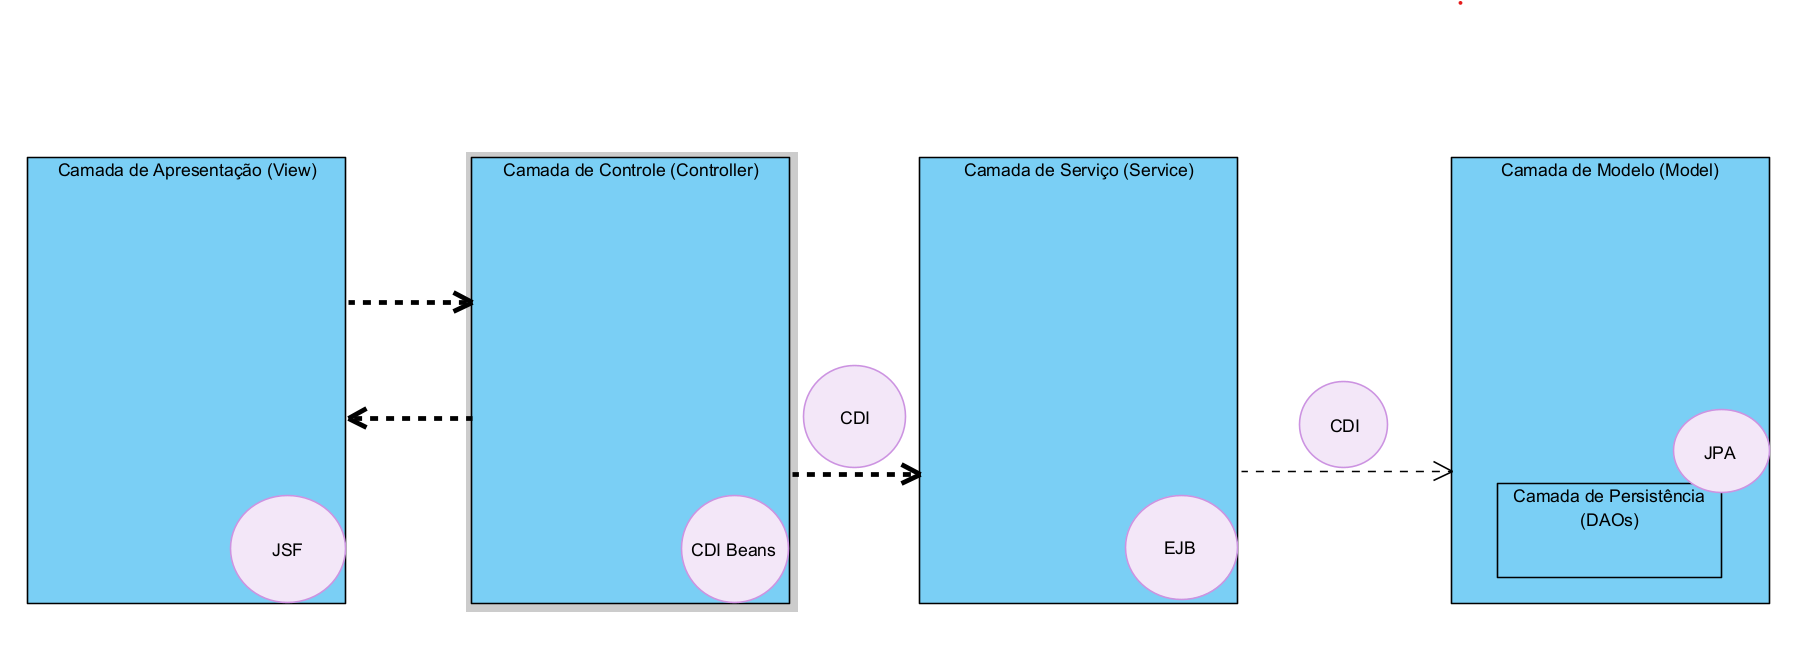
\includegraphics[width=0.8\textwidth]{figuras/arq.png}
	\caption{Arquitetura de Software.}
	\label{arq}
\end{figure}

A arquitetura utilizada será uma extensão do padrão MVC (Model-View-Controller), já consagrada pelas suas vantagens como: segregação de responsabilidades entre visualização, controle, lógica e persistência, trazendo clareza e eficiência no desenvolvimento e a reutilização de código via serviços e DAOs.

A arquitetura será organizada em 5 camadas principais, as quais seguem abaixo ao lado das suas respectivas tecnologias utilizadas:

\begin{itemize}
    \item Camada de Apresentação (View) - Páginas Web dinâmicas / Interface com o usuário – JSF
    \item Camada de Controle (Controller) – Controle de requisições - CDI Beans
    \item Camada de Serviço (Service) - Regras de Negócio – EJB
    \item Camada de Modelo (Model) – Entidades - JPA
    \item Camada de Persistência (DAO) – Acesso a dados - JPA
\end{itemize}



% \vitor{Substituir a Figura~\ref{arq} pelo diagrama UML da arquitetura do seu projeto e descrevê-la no texto. Caso use alguma arquitetura clássica, incluir referência bibliográfica com BibTeX (ex.:~\cite{fowler:book02}).}
